% !TEX root = ./Basilisk-inertialUKF-20190402.tex

\newpage

\section{Test Description and Success Criteria}

\subsection{Test 0: Individual Methods Tests}

The first test in this suite runs methods individually:

\begin{itemize}
\item{Read STMessages:} This test sends 3 ST messages in the wrong order (1.25s, 1s, 0.5s), and tests that the method organizes them chronologically relative to their timeTag. 
\item{Clean Update:} This test calls the Clean method and ensures previous sBar, covariance, and state values replaced the potentially erroneous current values. 
\item{Faulty Measurement Update:} This test gives a negative wM vector and ensures that the badUpdate is triggered
\item{Faulty Time Update:} The same test is run on the Time update
\item{Wheel acceleration in the inertial Prpagation:} This test compares the output array when the wheel acceleration is computed with expected values
\end{itemize}

\subsection{Test 1: StatePropInertialAttitude}

This test runs a pure propagation test. The states are set to a fixed value and integrated with the filter.
This shows filter stability in the simple case and a very low tolerance for error is permitted (1E-10). 

\subsection{Test 2: StatePropRateInertialAttitude}

This test runs a pure propagation test while adding gyro data. This ensures those messages are being read and used properly. 

\subsection{Test 3: StateUpdateInertialAttitude}

Given no dynamics, this test runs the filter by giving two star tracker messages. For the first half of the simulation, the measurements both read attitude values of $\bm \sigma =  \begin{bmatrix} 0.3 & 0.4 & 0.5 \end{bmatrix}$. After 1000s, the measurement changes to $\bm \sigma = \begin{bmatrix} 1.2 & 0 & 0 \end{bmatrix}$.

Figures \ref{fig:Test11} and \ref{fig:Test12} show the results for the states and covariance values. 
 \begin{figure}[htbp]\centerline{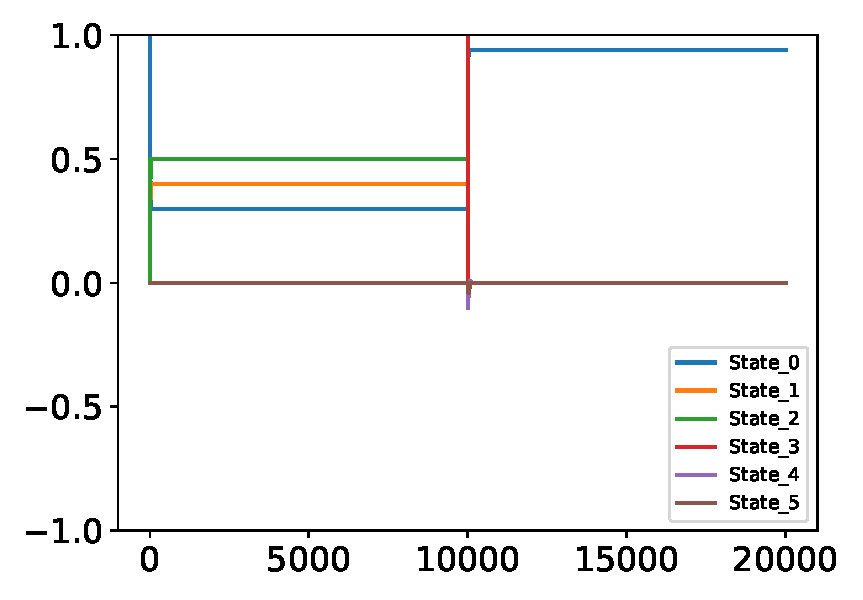
\includegraphics[width=0.9\textwidth, keepaspectratio]{AutoTeX/Test11}}\caption{Test 1 State convergence}\label{fig:Test11}\end{figure}
 \begin{figure}[htbp]\centerline{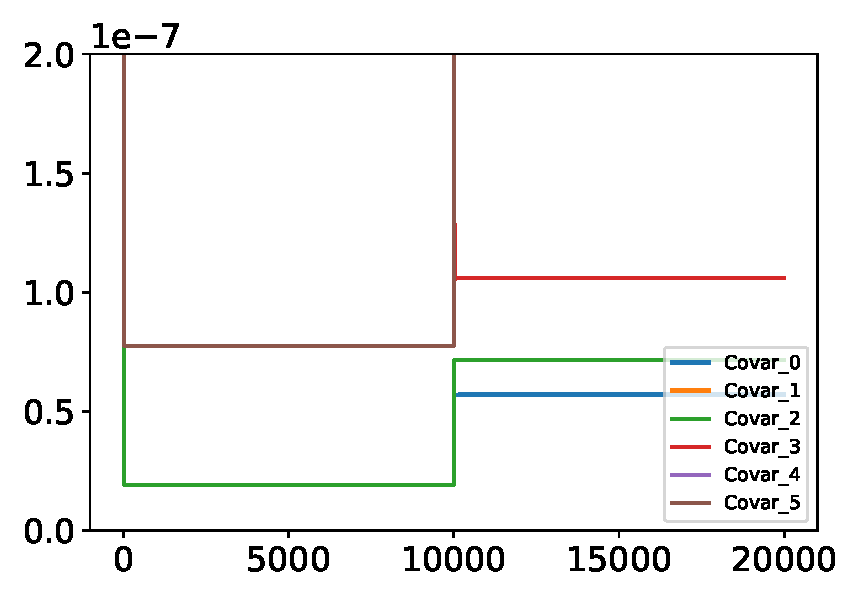
\includegraphics[width=0.9\textwidth, keepaspectratio]{AutoTeX/Test12}}\caption{Test 1 Covariance convergence}\label{fig:Test12}\end{figure}
 
\subsection{Test 4: StateUpdateRWInertialAttitude}

This last test runs the filter by giving two star tracker messages as well as reaction wheels. For the first half of the simulation, the measurements both read attitude values of $\bm \sigma = \begin{bmatrix} 0.3 & 0.4 & 0.5 \end{bmatrix}$. After 1000s, the measurement changes to $\bm \sigma = \begin{bmatrix} 1.2 & 0 & 0 \end{bmatrix}$. Wheel speeds are set to $\bm w_s = \begin{bmatrix} 0.1& 0.01& 0.1\end{bmatrix}$.

Figures \ref{fig:Test11} and \ref{fig:Test12} show the results for the states and covariance values. 
 \begin{figure}[htbp]\centerline{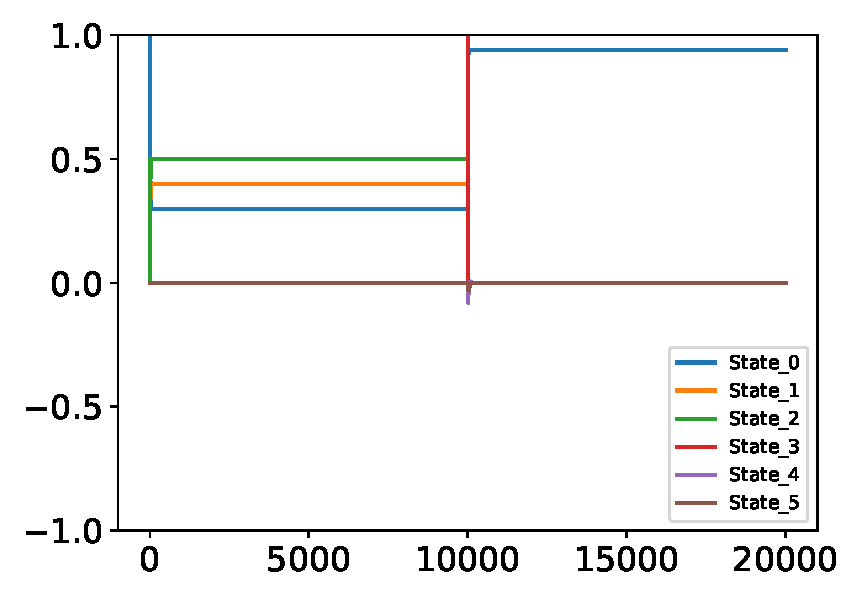
\includegraphics[width=0.7\textwidth, keepaspectratio]{AutoTeX/Test31}}\caption{Test 3 State convergence}\label{fig:Test31}\end{figure}
 \begin{figure}[htbp]\centerline{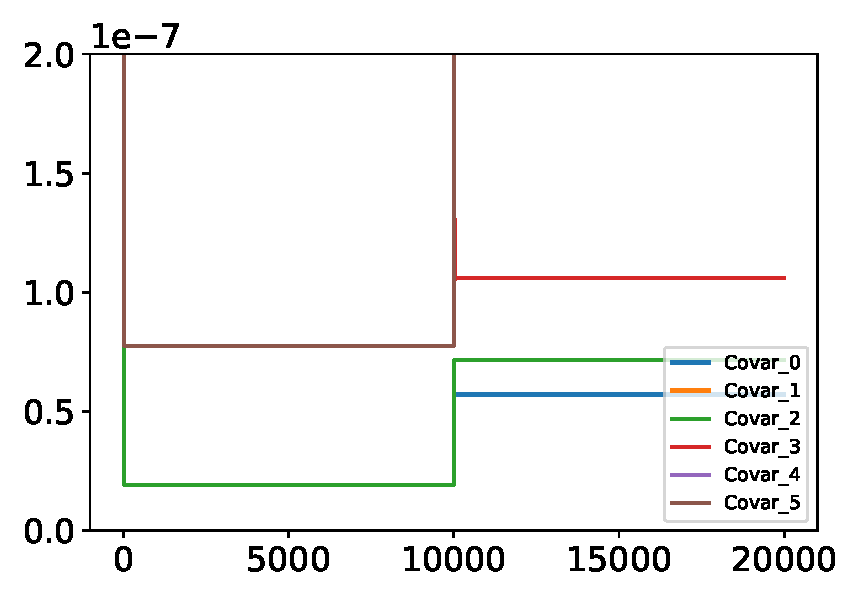
\includegraphics[width=0.7\textwidth, keepaspectratio]{AutoTeX/Test32}}\caption{Test 3 Covariance convergence}\label{fig:Test32}\end{figure}

\section{Test Parameters}

\begin{table}[ht]
\centering
\begin{tabular}{c|cc}
\hline
\hline
\textbf{Output Value Tested}     & \textbf{States Tolerated Error} & \textbf{Covariance Tolerated Error} \\ \hline
Test 0	        & 1e-10        		 &  N/A                   \\
%Test 1	        & \input{AutoTex/toleranceValue22}        		 &  N/A                   \\
%Test 2	   & \input{AutoTex/toleranceValue44}     			 &  Increase                           \\
Test 3	     & 1e-05     			 &  Increase                    \\
Test 4	 & 1e-05     			 &  N/A            		     \\\hline
\end{tabular}
\end{table}

\section{Test Results}

\begin{table}[H]
	\caption{Test results}
	\label{tab:results}
	\centering \fontsize{10}{10}\selectfont
	\begin{tabular}{c | c}
		\hline\hline
		\textbf{Check} 			&\textbf{Pass/Fail} \\ 
		\hline
	   Test 0	   			& \textcolor{ForestGreen}{PASSED} \\ 
%	   Test 1	   			& \textcolor{ForestGreen}{PASSED} \\ 
%	   Test 2	   			& \input{AutoTex/passFail44} \\ 
	   Test 3	   			& \textcolor{ForestGreen}{PASSED} \\ 
	   Test 4	   			& \textcolor{ForestGreen}{PASSED} \\ 
	   \hline\hline
	\end{tabular}
\end{table}
